\documentclass{article}
\usepackage[utf8]{inputenc}
\usepackage{amsmath}
\usepackage{listings}
\usepackage{geometry}
\usepackage{graphicx}
\usepackage{appendix}
\usepackage{subfig}
\usepackage{gensymb}
\usepackage{cancel}
\usepackage{physics}
\usepackage{empheq}
\usepackage{wrapfig}
\usepackage[colorlinks=true]{hyperref}
\usepackage{xcolor}
\definecolor{codegreen}{rgb}{0,0.6,0}
\definecolor{codegray}{rgb}{0.5,0.5,0.5}
\definecolor{codepurple}{rgb}{0.58,0,0.82}
\definecolor{backcolour}{rgb}{0.95,0.95,0.92}
\lstdefinestyle{mystyle}{
    backgroundcolor=\color{backcolour},   
    commentstyle=\color{codegreen},
    keywordstyle=\color{magenta},
    numberstyle=\tiny\color{codegray},
    stringstyle=\color{codepurple},
    basicstyle=\ttfamily\footnotesize,
    breakatwhitespace=false,         
    breaklines=true,                 
    captionpos=b,                    
    keepspaces=true,                 
    numbers=left,                    
    numbersep=5pt,                  
    showspaces=false,                
    showstringspaces=false,
    showtabs=false,                  
    tabsize=2
}

\lstset{style=mystyle}

\title{First Midterm}
\author{Simen Løken}
\date{October 2024}

\begin{document}

\maketitle
\renewcommand{\thesection}{Part \alph{section}}
\renewcommand{\thesubsection}{\alph{subsection})}

\section*{Contents}
This midterm contains parts a) through g), in addition to two appendices, A and B, which contain some Kronecker Delta contractions and diagrams respectively. Everything requested in the midterm should be answered unless I missed something, except the second quantization of the Hartree-Fock operator, which I could not find.
\newline
Repository with all code is at \href{https://github.com/simloken/FYS4480}{https://github.com/simloken/FYS4480}
\section{}
First, some formalism:
\newline
As we're dealing with hydrogen-like single-particle states, dealing with $n = 1, 2, 3$, we have that $m_l = 0$ with $l = 0$. Given that we're dealing with fermions, we know also that these states must have $s = \frac{1}{2}$. As such, we will represent the spins with the common representation $m_s = \pm \frac{1}{2} = \uparrow \downarrow$. \newline
As $l = 0$ and $m_l = 0$, we may represent the single particle states by only the quantum numbers $n, m_s$, and we get the generic form:
\begin{equation}
    | n m_s \rangle = a^\dagger _{n m_s} | 0 \rangle
\end{equation}
or more specifically, the six single particle states as:
\begin{gather*}
    | 1 \uparrow \rangle = a^\dagger_{1 \uparrow} |0 \rangle \\ 
    | 1 \downarrow \rangle = a^\dagger_{1 \downarrow} |0 \rangle \\
    | 2 \uparrow \rangle = a^\dagger_{2 \uparrow} |0 \rangle \\
    | 2 \downarrow \rangle = a^\dagger_{1 \downarrow} |0 \rangle \\
    | 3 \uparrow \rangle = a^\dagger_{3 \uparrow} |0 \rangle \\
    | 3 \downarrow \rangle = a^\dagger_{1 \downarrow} |0 \rangle
\end{gather*}
We may now move onto the ansatz for the ground state $|c\rangle = | \Phi_0 \rangle$, which is deceptively simple. \newline We select our ansatz for the ground state as the lowest energy state of our chosen basis, which becomes:
\begin{equation}
    | \Phi_0 \rangle = | 1\uparrow 1 \downarrow \rangle = a^\dagger_{1 \uparrow} a^\dagger_{1 \downarrow} | 0 \rangle 
\end{equation}
To better deal with the excitations of $| 0 \rangle$, we set $|\Phi_0 \rangle$ to be the Fermi level, which makes for less tedious work when constructing excited states as opposed to using $|0 \rangle$. We now (as suggested in the midterm) need to use particles and holes, of the form $| \Phi_i^\alpha \rangle$. Here, $i$ are the levels below the Fermi level (as defined above), and $\alpha$ are the particle states. When we say particles and holes, what we really mean is a filled state or a non-filled state, above or below the Fermi level respectively.
\newline
We can then define the generic form of $| \Phi_i^\alpha \rangle$ as:
\begin{equation} \label{gen}
    | \Phi_i^\alpha \rangle = a_\alpha^\dagger a_i | \Phi_0 \rangle
\end{equation}
Or more specifically the four states:
\begin{gather*}
    | \Phi_{1 \uparrow}^{2\uparrow} \rangle = a_{2 \uparrow}^\dagger a_{1\uparrow} | \Phi_0 \rangle \\
    | \Phi_{1 \downarrow}^{2\downarrow} \rangle = a_{2 \downarrow}^\dagger a_{1\downarrow} | \Phi_0 \rangle \\
    | \Phi_{1 \uparrow}^{3\uparrow} \rangle = a_{3 \uparrow}^\dagger a_{1\uparrow} | \Phi_0 \rangle \\
    | \Phi_{1 \downarrow}^{3\downarrow} \rangle = a_{3 \downarrow}^\dagger a_{1\downarrow} | \Phi_0 \rangle
\end{gather*}
which are the one-particle-one-hole excitations. Similarly, we may construct the two-particle-two-hole excitations by the generic form:
\begin{equation}
    | \Phi _{ij}^{a b} = a_a^\dagger a_b^\dagger a_i a_j |\Phi_0 \rangle
\end{equation}
Or again, more specifically:
\begin{gather*}
    | \Phi_{1\uparrow 1 \downarrow}^{2 \uparrow 2 \downarrow} \rangle = a_{2 \uparrow}^\dagger a_{2\downarrow}^\dagger a_{1 \uparrow} a_{1\downarrow} | \Phi_0 \rangle \\
    | \Phi_{1\uparrow 1 \downarrow}^{3 \uparrow 2 \downarrow} \rangle = a_{3 \uparrow}^\dagger a_{2\downarrow}^\dagger a_{1 \uparrow} a_{1\downarrow} | \Phi_0 \rangle \\
    | \Phi_{1\uparrow 1 \downarrow}^{2 \uparrow 3 \downarrow} \rangle = a_{2 \uparrow}^\dagger a_{3\downarrow}^\dagger a_{1 \uparrow} a_{1\downarrow} | \Phi_0 \rangle \\
    | \Phi_{1\uparrow 1 \downarrow}^{3 \uparrow 3 \downarrow} \rangle = a_{3 \uparrow}^\dagger a_{3\downarrow}^\dagger a_{1 \uparrow} a_{1\downarrow} | \Phi_0 \rangle
\end{gather*}
\section{}
We define $\hat H$ as a function of the creation and annihilation operators:
\begin{equation*}
    \hat H = \sum_{a b} \langle a | \hat h_0 | b \rangle a^\dagger_a a_b + \frac{1}{4} \sum_{abcd} \left(\langle a b| \hat v | cd \rangle - \langle a b | \hat v | d c \rangle \right) a^\dagger_a a^\dagger_b a_c a_d
\end{equation*}
which we will now use as a means of computing the expectation value of the ground state. To do this, we will employ a few tricks, namely from exercise 2 in week 38, that allowed us to rewrite respectively the definitions of $\hat H_0, \hat H_1$ in normal ordered form.
\newline
We have then:
\begin{equation*}
    \hat H_0 = \sum_{a b} \langle a | \hat h_0 | b \rangle a_a^\dagger a_b
\end{equation*}
\begin{equation*}
    \hat H_1  = \frac{1}{4} \sum_{abcd} \left(\langle a b | \hat v | c d \rangle - \langle a b | \hat v | d c \rangle \right) a^\dagger_a a^\dagger_b a_c a_d
\end{equation*}
which we rewrite respectively as:
\begin{equation}
    \hat H_0 = \sum_{a b} \langle a | \hat h_0 | b \rangle \{ a_a^\dagger a_b \} + \sum_i \langle i |\hat h_0 | i \rangle 
\end{equation}
\begin{equation}
    \hat H_1 = \frac{1}{4} \sum_{a b c d } \langle a b | \hat v | c d \rangle \{a_a^\dagger a_b^\dagger a_c a_d \} + \sum_{a b i} \langle a i | \hat v | b i \rangle \{ a_a^\dagger a_b \} + \frac{1}{2} \sum_{ij} \langle ij | \hat v| ij \rangle
\end{equation}
As it is now normal ordered, we can employ our second trick: Wick's Generalized Theorem. Given that $\hat H$ is normal ordered, we then have that the squigly-bracketed terms (that is $\{a_a^\dagger a_b\}$ and $\{a_a^\dagger a_b^\dagger a_c a_d \}$) become zero, giving:
\begin{equation*}
    E\left[\Phi_0 \right] = \langle \Phi_0 | \hat H | \Phi_0 \rangle
\end{equation*}
where we find the expectation values of $\hat H_0$ and $\hat H_1$ to be:
\begin{equation*}
    \langle \Phi_0 | \hat H_0 | \Phi_0 \rangle = \sum_i \langle i | \hat h_0 | i \rangle
\end{equation*}
\begin{equation*}
    \langle \Phi_0 | \hat H_1 | \Phi_0 \rangle = \frac{1}{2} \sum_{ij} \langle ij | \hat v | ij \rangle - \langle ij | \hat v | ji \rangle
\end{equation*}
Giving finally the requested expression for the ground state:
\begin{equation}
    E\left[\Phi_0 \right] = \sum_i \langle i | \hat h_0 | i \rangle + \frac{1}{2} \sum_{ij} \langle ij | \hat v | ij \rangle - \langle ij | \hat v | ji \rangle
\end{equation}
the only difference being we have exchanged $1/r$ for $\hat v$ for readability.
\newline
We now wish to evaluate this expression as a function of Z. 
\newline
We start at:
\begin{equation*}
    E\left[\Phi_0 \right] = \sum_i \langle i | \hat h_0 | i \rangle + \frac{1}{2} \sum_{ij} \langle ij | \hat v | ij \rangle - \langle ij | \hat v | ji \rangle
\end{equation*}
from which we get:
\begin{gather*}
    E\left[\Phi_0 \right] = \langle 1 \uparrow | \hat h_0 | 1 \uparrow \rangle + \langle 1 \downarrow | \hat h_0 | 1 \downarrow \rangle + \frac{1}{2}( \langle 1 \uparrow 1 \downarrow | \hat v | 1 \uparrow 1 \downarrow \rangle - \langle 1 \uparrow 1 \downarrow | \hat v | 1 \downarrow 1 \uparrow \rangle  \\ + \langle 1 \downarrow 1 \uparrow 1 \hat v | 1 \downarrow 1 \uparrow \rangle - \langle 1 \downarrow 1 \uparrow | \hat v | 1 \uparrow 1 \downarrow \rangle )
\end{gather*}
Here, the last term on both lines of the equation becomes 0, and thus we get:
\begin{equation}
    E\left[\Phi_0 \right] = 2 \langle 1 | \hat h_0 | 1 \rangle + \langle 11 | \hat v | 11 \rangle
\end{equation}
We look at the table given in the exercise and find that $\langle 11 | \hat v | 11 \rangle = \frac{5Z}{8}$, giving us:
\begin{equation}
    E\left[\Phi_0 \right] = - {Z^2} + \frac{5Z}{8}¨\xrightarrow[]{Z = 2} E\left[\Phi_0 \right] = - \frac{11}{4} \; a.u.
\end{equation}
\section{}
The natural place to start is to find a term for $\langle \Phi_0 | \hat H | \Phi_i^\alpha \rangle$. If we rewrite the term as:
\begin{equation*}
    \langle \Phi_0 | \hat H | \Phi_i^\alpha \rangle = \langle \Phi_0 | \hat H a_a^\dagger a_i | \Phi_0 \rangle
\end{equation*}
Then we may again use Wick's Generalized Theorem, and we find that:
\begin{equation*}
    \langle \Phi_0 | \hat H | \Phi_i^\alpha \rangle = \sum_{ab} \langle a | \hat h_0 | b \rangle \langle \Phi_0 | \{ a_a^\dagger a_b \} | \Phi_i^\alpha \rangle + \sum_{abj} (\langle pj | \hat v | q j \rangle - \langle pj | \hat v | jq \rangle) \langle \Phi_0 | \{ a_a^\dagger a_b \} | \Phi_i^\alpha \rangle
\end{equation*}
Notice the term $\langle \Phi_0 | \{ a_a^\dagger a_b \} | \Phi_i^\alpha \rangle$, which is present in both terms. We may rewrite this as:
\begin{equation*}
    \langle \Phi_0 | \{ a_a^\dagger a_b \} | \Phi_i^\alpha \rangle = \delta_{ai} \delta_{b \alpha}
\end{equation*}
from which we get the much neater form:
\begin{equation}
    \langle \Phi_0 | \hat H | \Phi_i^\alpha \rangle = \langle i | \hat h_0 | \alpha \rangle + \sum_j \langle ij | \hat v | \alpha j \rangle - \langle ij | \hat v | j \alpha \rangle
\end{equation}
We wish now to find the expression for all one-particle-one-hole states, which we may write as:
\begin{equation*}
    \langle \Phi_i^\alpha | \hat H | \Phi_j^\beta \rangle = \langle \Phi_0 | a_i^\dagger a_\alpha \hat H a_b^\dagger a_j | \Phi_0 \rangle
\end{equation*}
which becomes for $H_0$ and $H_1$ respectively:
\begin{gather*}
    \langle \Phi_i^\alpha | \hat H_0 | \Phi_j^\beta \rangle = \sum_{ab} \langle a | \hat h_0 | b \rangle \left(\{a_i^\dagger a_\alpha \} \{a_a^\dagger a_b \} \{a_\beta^\dagger a_j \} \right) \\ 
    + \sum_k \langle k | \hat h_0 | k \rangle \left(\{a_i^\dagger a_\alpha \} \{a_\beta^\dagger a_j \} \right)
\end{gather*}
\begin{gather*}
    \langle \Phi_i^\alpha | \hat H_1 | \Phi_j^\beta \rangle = \frac{1}{4} \sum_{abcd} \left(\langle ab | \hat v | cd \rangle - \langle ab | \hat v | dc \rangle \right) \left(\{a_i^\dagger a_\alpha \} \{a_a^\dagger a_b^\dagger a_d a_c \} \{a_\beta^\dagger a_j \} \right) \\
    + \sum_{abk} \left\langle a k | \hat v | b k \rangle - \langle a k | \hat v | k b \rangle \right) \left(\{a_i^\dagger a_\alpha \} \{a_a^\dagger a_b \} \{a_\beta^\dagger a_j \} \right) \\
    + \sum_{kl} \left(\langle kl | \hat v | kl \rangle - \langle kl | \hat v | lk \rangle \right) \left(\{a_i^\dagger a_\alpha \} \{a_\beta^\dagger a_j \} \right)
\end{gather*}
Again, we may contract these terms, giving a much neater (see \ref{kron} for a more robust derivation of the term below):
\begin{equation}
    \langle \Phi_i^\alpha | \hat H_0 | \Phi_j^\beta \rangle = \langle \alpha | \hat h_0 | \beta \rangle \delta_{ij} - \langle j | \hat h_0 | i \rangle \delta_{\alpha \beta} + \sum_k \langle k | \hat h_0 | k \rangle \delta_{ij} \delta_{\alpha \beta}
\end{equation}
\begin{equation}
    \begin{split}
    \langle \Phi_i^\alpha | \hat H_1 | \Phi_j^\beta \rangle &= \langle \alpha j | \hat v | i \beta \rangle - \langle \alpha j | \hat v | \beta i \rangle \\
    &+ \sum_k \left(\left( \langle \alpha k | \hat v | \beta k \rangle - \langle \alpha k | \hat v | k \beta \rangle \right) \delta_{ij} - \left(\langle j k | \hat v | ik \rangle - \langle j k| \hat v |  ki \rangle \right)\delta_{\alpha \beta}\right) \\ 
    &+ \frac{1}{2} \sum_{kl}\left( \langle k l | \hat v | kl \rangle - \langle k l | \hat v | lk \rangle \right)\delta_{ij}\delta_{\alpha\beta}
    \end{split}
\end{equation}
The Hamiltonian Matrix is now:
\begin{equation}
\hat H_{mat} = 
\begin{bmatrix}
\langle \Phi_0 | \hat H | \Phi_0 \rangle & 
\langle \Phi_{0} | \hat H | \Phi_{1\uparrow}^{2\downarrow} \rangle &
\langle \Phi_0 | \hat H | \Phi_{1\downarrow}^{2\downarrow} \rangle & 
\langle \Phi_0 | \hat H | \Phi_{1\uparrow}^{3\uparrow} \rangle &
\langle \Phi_0 | \hat H | \Phi_{1\downarrow}^{3\downarrow} \rangle \\

\langle \Phi_{1\uparrow}^{2\uparrow} | \hat H | \Phi_0 \rangle & 
\langle \Phi_{1\uparrow}^{2\uparrow} | \hat H | \Phi_{1\uparrow}^{2\downarrow} \rangle &
\langle \Phi_{1\uparrow}^{2\uparrow} | \hat H | \Phi_{1\downarrow}^{2\downarrow} \rangle & 
\langle \Phi_{1\uparrow}^{2\uparrow} | \hat H | \Phi_{1\uparrow}^{3\uparrow} \rangle &
\langle \Phi_{1\uparrow}^{2\uparrow} | \hat H | \Phi_{1\downarrow}^{3\downarrow} \rangle \\

\langle \Phi_{1\downarrow}^{2\downarrow} | \hat H | \Phi_0 \rangle & 
\langle \Phi_{1\downarrow}^{2\downarrow} | \hat H | \Phi_{1\uparrow}^{2\downarrow} \rangle &
\langle \Phi_{1\downarrow}^{2\downarrow} | \hat H | \Phi_{1\downarrow}^{2\downarrow} \rangle & 
\langle \Phi_{1\downarrow}^{2\downarrow} | \hat H | \Phi_{1\uparrow}^{3\uparrow} \rangle &
\langle \Phi_{1\downarrow}^{2\downarrow} | \hat H | \Phi_{1\downarrow}^{3\downarrow} \rangle \\

\langle \Phi_{1\uparrow}^{3\uparrow} | \hat H | \Phi_0 \rangle & 
\langle \Phi_{1\uparrow}^{3\uparrow} | \hat H | \Phi_{1\uparrow}^{2\downarrow} \rangle &
\langle \Phi_{1\uparrow}^{3\uparrow} | \hat H | \Phi_{1\downarrow}^{2\downarrow} \rangle & 
\langle \Phi_{1\uparrow}^{3\uparrow} | \hat H | \Phi_{1\uparrow}^{3\uparrow} \rangle &
\langle \Phi_{1\uparrow}^{3\uparrow} | \hat H | \Phi_{1\downarrow}^{3\downarrow} \rangle \\

\langle \Phi_{1\downarrow}^{3\downarrow} | \hat H | \Phi_0 \rangle & 
\langle \Phi_{1\downarrow}^{3\downarrow} | \hat H | \Phi_{1\uparrow}^{2\downarrow} \rangle &
\langle \Phi_{1\downarrow}^{3\downarrow} | \hat H | \Phi_{1\downarrow}^{2\downarrow} \rangle & 
\langle \Phi_{1\downarrow}^{3\downarrow} | \hat H | \Phi_{1\uparrow}^{3\uparrow} \rangle &
\langle \Phi_{1\downarrow}^{3\downarrow} | \hat H | \Phi_{1\downarrow}^{3\downarrow} \rangle \\
\end{bmatrix}
\end{equation}
Performing now the calculation with the python script, we find that such an approach yields the energy $E^{He}_{Mat} = -2.77\; a.u.$ which is a relatively good measurement.
\section{}
We use the same approach as we did for Helium, and the same basis, except that we're now dealing with $Z=4$. Thus we get the ansatz:
\begin{equation}
    |\Phi_0\rangle = a_{1\uparrow}^\dagger a_{1\downarrow}^\dagger a_{2\uparrow}a_{2\downarrow}|0\rangle
\end{equation}
And we again get the same generic form from Eq. [\ref{gen}] and the specific states:
\begin{gather*}
    |\Phi_{1\uparrow}^{3\uparrow} = a_{3\uparrow}^\dagger a_{1\uparrow} |\Phi_0 \rangle \\
    |\Phi_{1\downarrow}^{3\downarrow} = a_{3\downarrow}^\dagger a_{1\downarrow} |\Phi_0 \rangle \\
    |\Phi_{2\uparrow}^{3\uparrow} = a_{3\uparrow}^\dagger a_{2\uparrow} |\Phi_0 \rangle \\
    |\Phi_{2\downarrow}^{3\downarrow} = a_{3\uparrow}^\dagger a_{2\downarrow} |\Phi_0 \rangle
\end{gather*}
and we end up with:
\begin{equation*}
    E[\Phi_0] = \sum_i \langle i | \hat h_0 | i \rangle + \langle 11 | V | 11 \rangle + \langle 22 | V | 22 \rangle + 2\left(\langle 12 | V | 12 \rangle + \langle 21 | V | 21 \rangle\right) - \left(\langle 12|V|21\rangle + \langle 21|V| 12 \rangle \right)
\end{equation*}
\begin{equation}
    E[\Phi_0] = - \frac{5Z^2}{4} + \frac{586373}{373248}Z \xrightarrow[]{Z = 4} E\left[\Phi_0 \right] = -13.716 \; a.u.
\end{equation}
We perform now again the same calculation as in c), except that we now move the Fermi level up 1. We find then the energy $E_{Mat}^{Be} = -13.75 a.u.$, which is a small improvement from the rudimentary value we found just above.
\section{}
We must now rewrite our expression for the ground state estimation, we have that:
\begin{equation*}
    E[\Phi_0^{\mathcal{H}\mathcal{F}}] = \sum_i \langle i | \hat h_0 | i \rangle + \frac{1}{2} \sum_{ij} \langle ij | \hat v | ij \rangle - \langle ij | \hat v | ji \rangle
\end{equation*}
Note that we here have swapped basis. We denote our old basis by greek letters $\alpha \beta $ etc.. Our new basis uses roman letters $i, j$ and so forth. We may then rewrite in terms of our old basis:
\begin{equation*}
    E[\Phi_0^{\mathcal{H}\mathcal{F}}] = \sum_i \sum_{\alpha \beta} C_{i\alpha}^* C_{i \beta}^* \langle \alpha | \hat h_0 | \beta \rangle + \frac{1}{2} \sum_{ij}\sum_{\alpha \beta \gamma \delta}C_{i\alpha}^* C_{j\beta}^* C_{i\gamma} C_{j\delta} \left(\langle \alpha \beta | \hat v | \gamma \delta \langle - \langle \alpha \beta | \hat v | \delta \gamma \rangle \right)
\end{equation*}
We know that our new single particle basis is orthonormal, that is:
\begin{equation*}
    \langle a | b \rangle = \delta_{a b} = \sum_{\alpha\beta} C_{a \alpha}^* C_{a \beta} \langle \alpha | \beta \rangle = \sum_\alpha C_{a \alpha}^* C_{a \alpha}
\end{equation*}
and thus we write our functional to minimize:
\begin{equation}
    \mathcal{F}[\Phi_0^{\mathcal{H}\mathcal{F}}] = E[\Phi_0^{\mathcal{H}\mathcal{F}}] - \sum_i \epsilon_i \sum_\alpha C_{i\alpha}^* C_{i \alpha}
\end{equation}
where $\epsilon_i$ are our Lagrange multipliers.\newline
We can now minimize $\mathcal{F}$ with respect to $C_{i \alpha}^*$, and thus we must solve:
\begin{equation*}
    \frac{\partial}{\partial C_{i \alpha}^*} \mathcal{F}[\Phi_0^{\mathcal{H}\mathcal{F}}] = \frac{\partial}{\partial C_{i \alpha}^*} \left( E[\Phi_0^{\mathcal{H}\mathcal{F}}] - \sum_j \epsilon_j \sum_a C_{j \alpha}^* C_{j \alpha} \right) = 0
\end{equation*}
This can look quite intimidating, but if we take it one term at a time, it's not \emph{that} bad. Let us start at the beginning with $E[\Phi_0^{\mathcal{H}\mathcal{F}}]$, which is made up of two terms, the one-body and two-body contribution respectively. The one-body is simple, giving:
\begin{equation*}
    \frac{\partial}{\partial C_{i \alpha}^*} \sum_i \sum_{\alpha \beta} C_{i\alpha}^* C_{i \beta}^* \langle \alpha | \hat h_0 | \beta \rangle = \sum_\beta C_{i\beta} \langle \alpha | \hat h_0 | \beta \rangle
\end{equation*}
and the two-body is a step up, giving:
\begin{equation*}
    \frac{\partial}{\partial C_{i \alpha}^*}\frac{1}{2} \sum_{ij}\sum_{\alpha \beta \gamma \delta}C_{i\alpha}^* C_{j\beta}^* C_{i\gamma} C_{j\delta} \left(\langle \alpha \beta | \hat v | \gamma \delta \langle - \langle \alpha \beta | \hat v | \delta \gamma \rangle \right) = \sum_j \sum_{\beta \gamma \delta} C_{j \beta}^* C_{i\gamma} C_j{\delta} \left(\langle \alpha \beta | \hat v | \gamma \delta \rangle - \langle \alpha \beta | \hat v | \delta \gamma \rangle \right)
\end{equation*}
We are now finally left with only the Lagrange multiplier term of $\mathcal{F}$, which is:
\begin{equation*}
    \frac{\partial}{\partial C_[i \alpha]^*} \sum_i \epsilon_i \sum_\alpha C_{i\alpha}^* C_{i \alpha} = \epsilon_i C_{i \alpha}
\end{equation*}
Although selecting $\epsilon$ as our Lagrange multiplier (as opposed to the more normal $\lambda$) may have been "cheating" in the sense that it makes the connection easier to see, it is now trivial to see with these three terms where this is going. Namely we have:
\begin{equation}
    \frac{\partial}{\partial C_{i \alpha}^*} \mathcal{F}[\Phi_0^{\mathcal{H}\mathcal{F}}] = \sum_\beta C_{i\beta} \langle \alpha | \hat h_0 | \beta \rangle + \sum_j \sum_{\beta \gamma \delta} C_{j \beta}^* C_{i\gamma} C_j{\delta} \left(\langle \alpha \beta | \hat v | \gamma \delta \rangle - \langle \alpha \beta | \hat v | \delta \gamma \rangle \right) - \epsilon_i C_{i \alpha} = 0
\end{equation}
Which is:
\begin{equation*}
    \sum_\beta C_{i\beta} \langle \alpha | \hat h_0 | \beta \rangle + \sum_j \sum_{\beta \gamma \delta} C_{j \beta}^* C_{i\gamma} C_j{\delta} \left(\langle \alpha \beta | \hat v | \gamma \delta \rangle - \langle \alpha \beta | \hat v | \delta \gamma \rangle \right) = \epsilon_i C_{i \alpha}
\end{equation*}
We're now only missing one step, inserting the expression for $h^{\mathcal{H}\mathcal{F}}$ given. It is quite trivial to see that if:
\begin{equation*}
    h_{\alpha\beta}^{\mathcal{H}\mathcal{F}} = \left[\langle \alpha| \hat h_0 | \beta \rangle + \sum_j \sum_{\gamma \delta} C_{j\gamma}^* C_{j\delta} \left( \langle \alpha \gamma | \hat v | \beta \delta \rangle - \langle \alpha \gamma | \hat v | \delta \beta \rangle \right) \right]
\end{equation*}
we can then pull out the summation over $\beta$, giving:
\begin{equation*}
    \sum_\beta \left[\langle \alpha| \hat h_0 | \beta \rangle + \sum_j \sum_{\gamma \delta} C_{j\gamma}^* C_{j\delta} \left( \langle \alpha \gamma | \hat v | \beta \delta \rangle - \langle \alpha \gamma | \hat v | \delta \beta \rangle \right) \right] = \epsilon_i C_{i\alpha}
\end{equation*}
Finally giving us:
\begin{equation}
    \sum_\beta h_{\alpha\beta}^{\mathcal{H}\mathcal{F}} = \epsilon_i C_{i \alpha}
\end{equation}
as requested. 
\newline
No idea how to find the second quantization.
\section{}
We use the single particle orbits in our Hartree-Fock code to find the diagonalization:
\begin{gather*}
    \epsilon_1^{He} = -0.783 \\ 
    \epsilon_2^{He} = -0.783 \\
    \epsilon_3^{He} = 0.040 \\
    \epsilon_4^{He} = 0.040 \\
    \epsilon_5^{He} = 0.453 \\
    \epsilon_6^{He} = 0.453
\end{gather*}
and
\begin{gather*}
    \epsilon_1^{Be} = -3.951 \\
    \epsilon_2^{Be} = -3.951 \\
    \epsilon_3^{Be} = -0.104 \\
    \epsilon_4^{Be} = -0.104 \\
    \epsilon_5^{Be} = 0.866 \\
    \epsilon_6^{Be} = 0.866
\end{gather*}
Additionally, after one iteration of our Hartree-Fock code we find that $E_0^{He} = -2.83\;a.u.$ and $E_0^{Be} = -14.50 \;a.u.$
\newpage
\section{}
We extend our approach from above to be an iterative one. The most sensible way to do this is to continually measure the slope of our convergence, and whenever it is lower than some tolerance we end the calculation. \newline
To do this, we take the norm of the density matrix eigenvalues $\epsilon$, as:
\begin{equation*}
    \delta_{tol} > \frac{|\epsilon_{new} - \epsilon_{old}|}{N}
\end{equation*}
where $\epsilon_{new}$ are our current eigenvalues, and $\epsilon_{old}$ are our old values. Other alternatives could be looking at the ground state energy or using a rolling average, although a rolling average is better served for volatile systems/problems, which this is not.
\newline
When we let our system iterate with a tolerance of $1 \times 10^{-15}$, we find that our system converges after 19 and 20 iterations respectively. We find the energies to be almost the exact same as the non-iterative version of the Hartree-Fock code, at $E_0^{He} = -2.83\;a.u.$ and $E_0^{Be} = -14.51 \;a.u.$ respectively.
\newline
\begin{figure}[ht!]
    \centering
    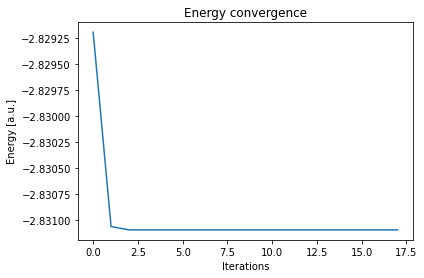
\includegraphics[scale=0.35]{convergence_He.png}
    \caption{The convergence of our Hartree-Fock Algorithm for Helium}
    \label{fig:enter-label}
\end{figure}
\begin{figure}[ht!]
    \centering
    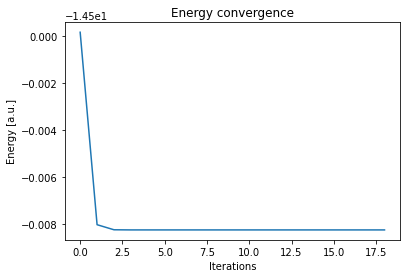
\includegraphics[scale=0.35]{convergence_Be.png}
    \caption{The convergence of our Hartree-Fock Algorithm for Beryllium}
    \label{fig:enter-label}
\end{figure}
\newpage
Lastly, let us review all our results and discuss them for a little bit, we found the following:
\begin{table}[h!]
    \centering
    \caption{Energy Values for Helium and Beryllium for each method}
    \begin{tabular}{@{}lcc@{}}
        \toprule
        Method & Helium (He) [a.u.] & Beryllium (Be) [a.u.] \\ \midrule
        $E$         & -2.91     & -14.67    \\
        $E_{gs}$    & -2.75     & -13.72    \\
        $E_{Mat}$   & -2.77     & -13.75    \\
        $E_{HF1}$   & -2.83     & -14.50    \\
        $E_{HF}$    & -2.83     & -14.51    \\ \bottomrule
    \end{tabular}
    \label{tab:energy_values}
\end{table}
\newline
We find, perhaps somewhat unsurprisingly, that there is an upwards trend in our results as we either improve or further increase the 'complexity' of our models. This is as expected. It should however be noted that there might be something wrong with the Hartree-Fock method, as I believe we should be seeing more improvement that the very miniscule percent we're seeing after 20 or so iterations. 
\renewcommand{\thesection}{Appendix \Alph{section}}
\setcounter{section}{0}
\newpage
\section{- \;Contractions: Kronecker-Deltas} \label{kron}
The contractions made in part c) may feel a little too hand-wavy, so here are the complete derivation of the Kronecker-Deltas:
\begin{figure}[ht!]
    \centering
    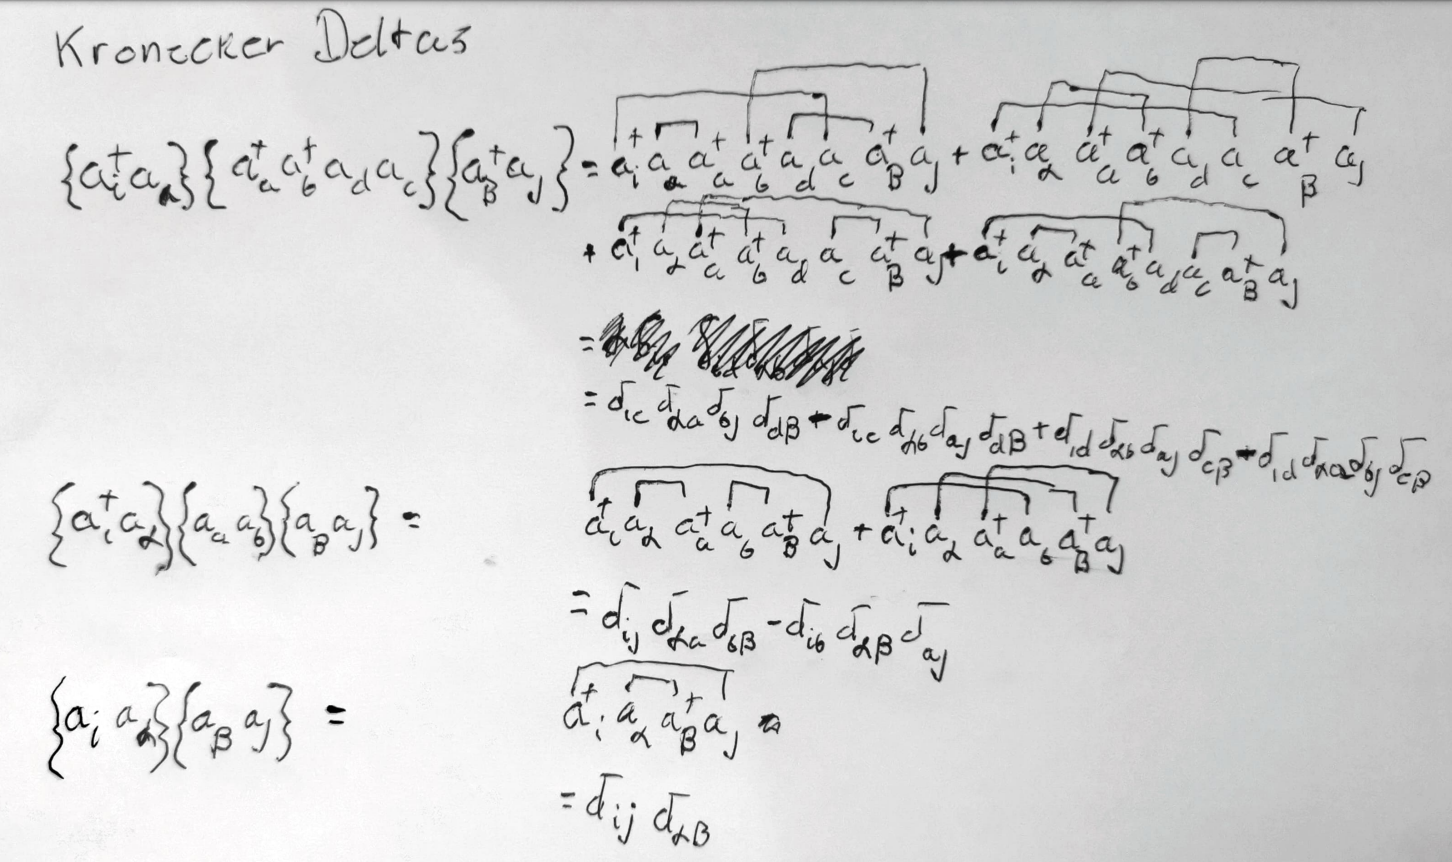
\includegraphics[scale=0.4]{kronecker.PNG}
    \caption{Kronecker Deltas for c)}
    \label{fig:enter-label}
\end{figure}
\newpage
\section{- \;Diagrams}
The diagrams can be found here:
\subsection*{$\langle \theta_0 | \hat H | \theta_i^\alpha\rangle$ Diagram}
\begin{figure}[ht!]
    \centering
    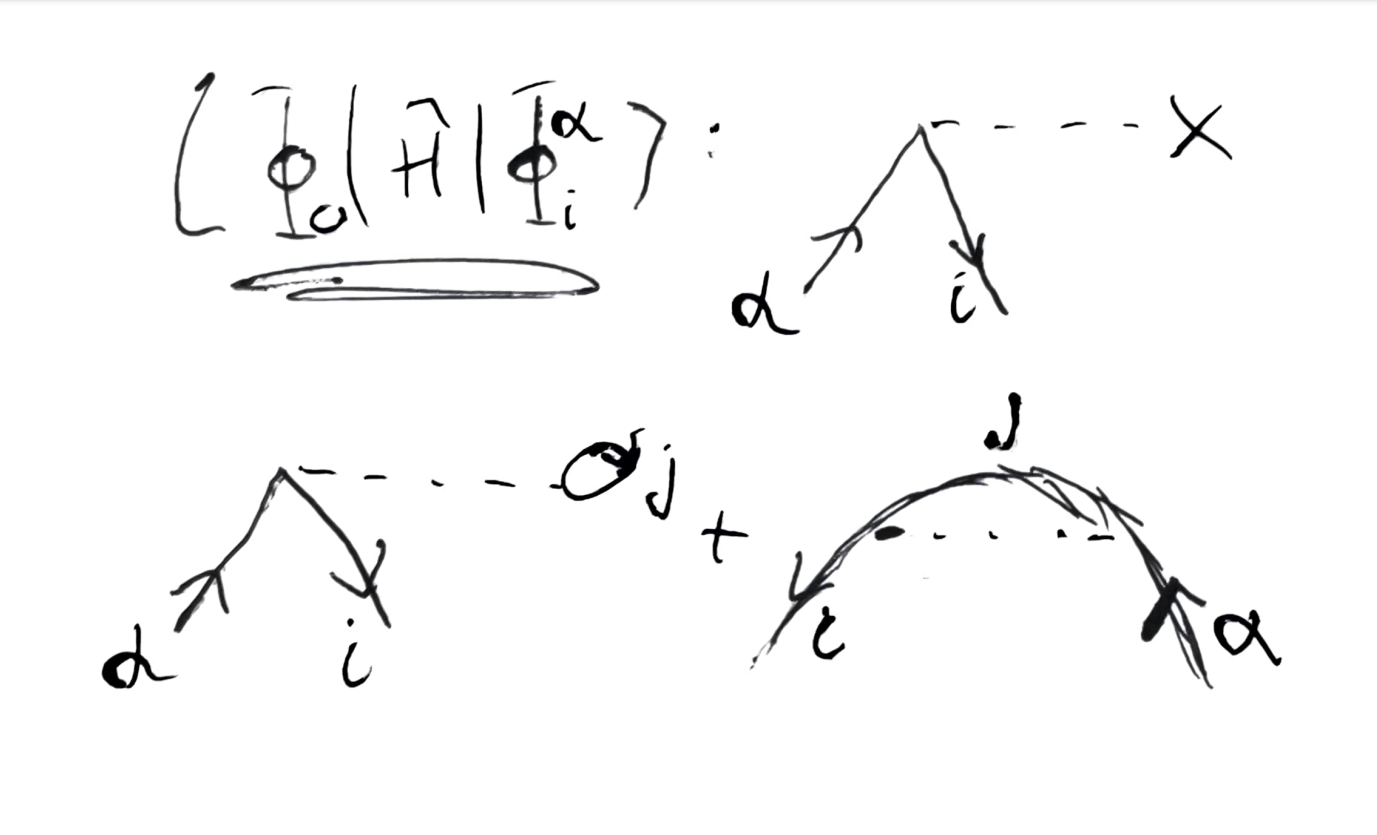
\includegraphics[scale=0.4]{diagram_1.PNG}
    \caption{Diagrams for $\langle \Phi_0 | \hat H | \Phi_i^\alpha \rangle$}
    \label{fig:enter-label}
\end{figure}
\newpage
\subsection*{$\langle \theta_i^\alpha | \hat H | \theta_i^\beta\rangle$ Diagram}
\begin{figure}[ht!]
    \centering
    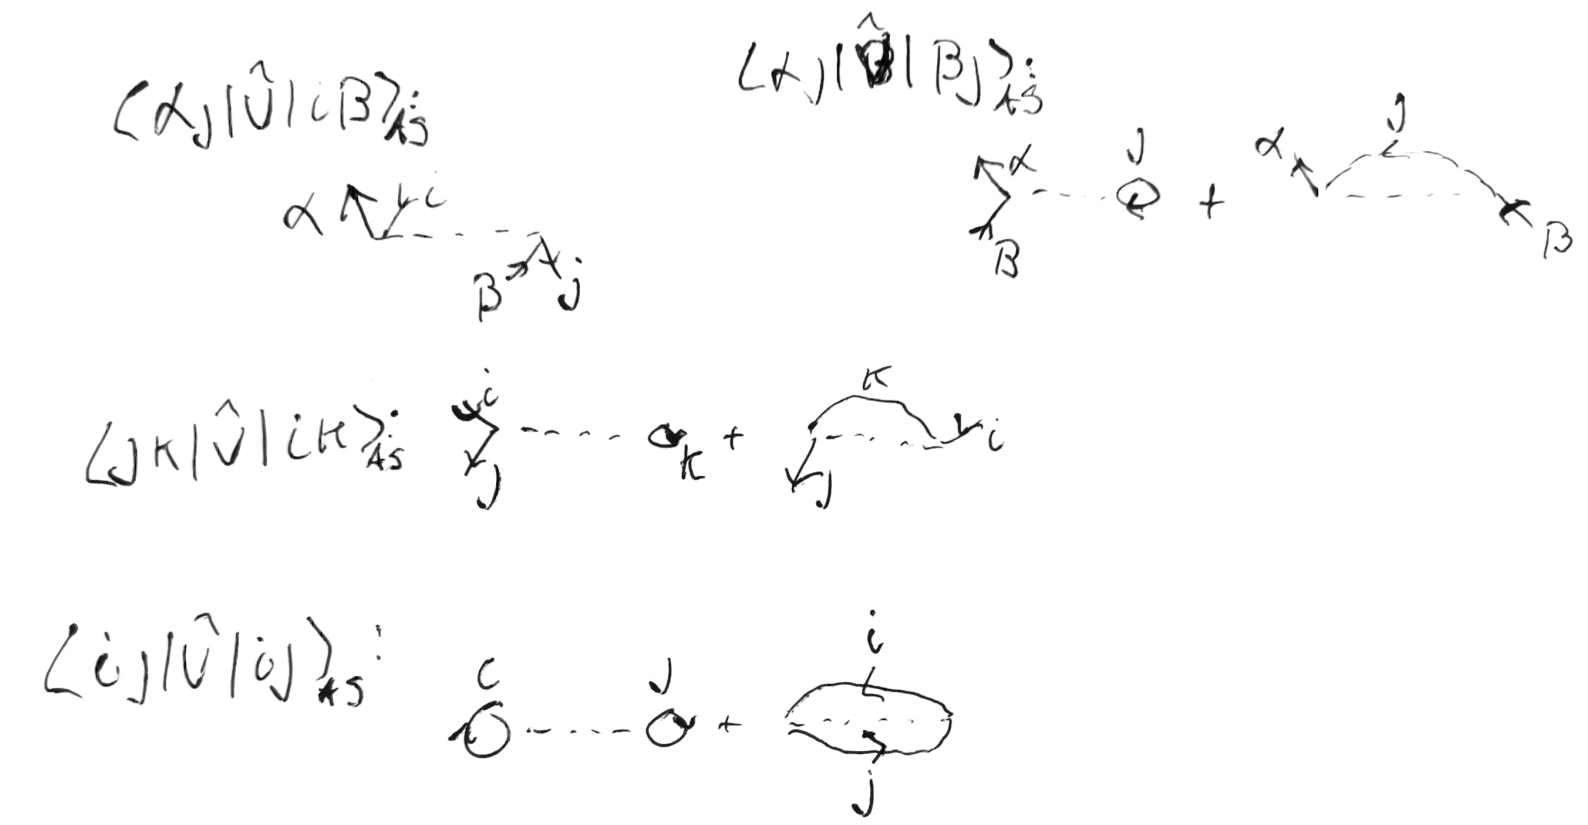
\includegraphics[scale=0.4]{diagram_2.PNG}
    \caption{Diagrams for $\langle \Phi_i^\alpha | \hat H | \Phi_j^\beta\rangle$}
    \label{fig:enter-label}
\end{figure}
\newpage
\subsection*{$h_{\alpha\beta}^{\mathcal{H}\mathcal{F}}$ Diagram}
\begin{figure}[ht!]
    \centering
    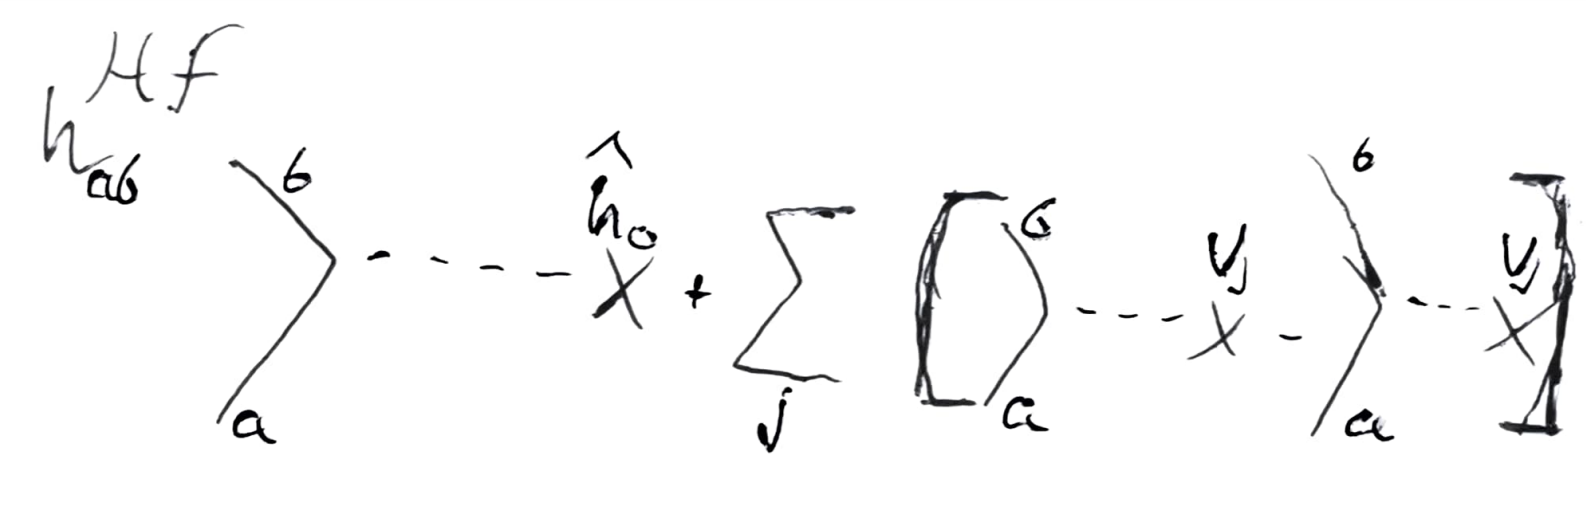
\includegraphics[scale=0.4]{diagram_hartree_fock.PNG}
    \caption{Diagram for Hartree Fock}
    \label{fig:enter-label}
\end{figure}

\end{document}
